\documentclass[12pt,letterpaper]{article}

\usepackage{fullpage}
\usepackage{lscape}
\usepackage{gantt}
\usepackage{booktabs}
\usepackage{colortbl}
\usepackage{titlesec}
\usepackage{tabularx}
\usepackage{hyperref}
\usepackage{graphicx}

\begin{document}

\begin{center}
	{\bf\Large Oregon State University \\
          Autonomous Aerial Robotics Team \\
          2014 Project Proposal
	  \\ [1em]
	}

        {\small
          Kyle Cesare, \url{cesarek@onid.orst.edu}
        }
\end{center}

% TODO:
%  - Mistakes made last year, how to correct this year

\begin{abstract}
The Oregon State University Autonomous Aerial Robotics Team builds autonomous
aerial vehicles to compete in the International Aerial Robotics Competition. The
competition is structured to push the current capabilities of autonomous aerial
vehicles. The team joins computer scientists, electrical engineers, and
mechanical engineers to design, build, and program these aerial vehicles from
start to finish. It is a great learning experience for everyone involved. The
team participates in a number of outreach events to teach the community about
robotics.  \end{abstract}

\begin{figure}[h]
  \centering
  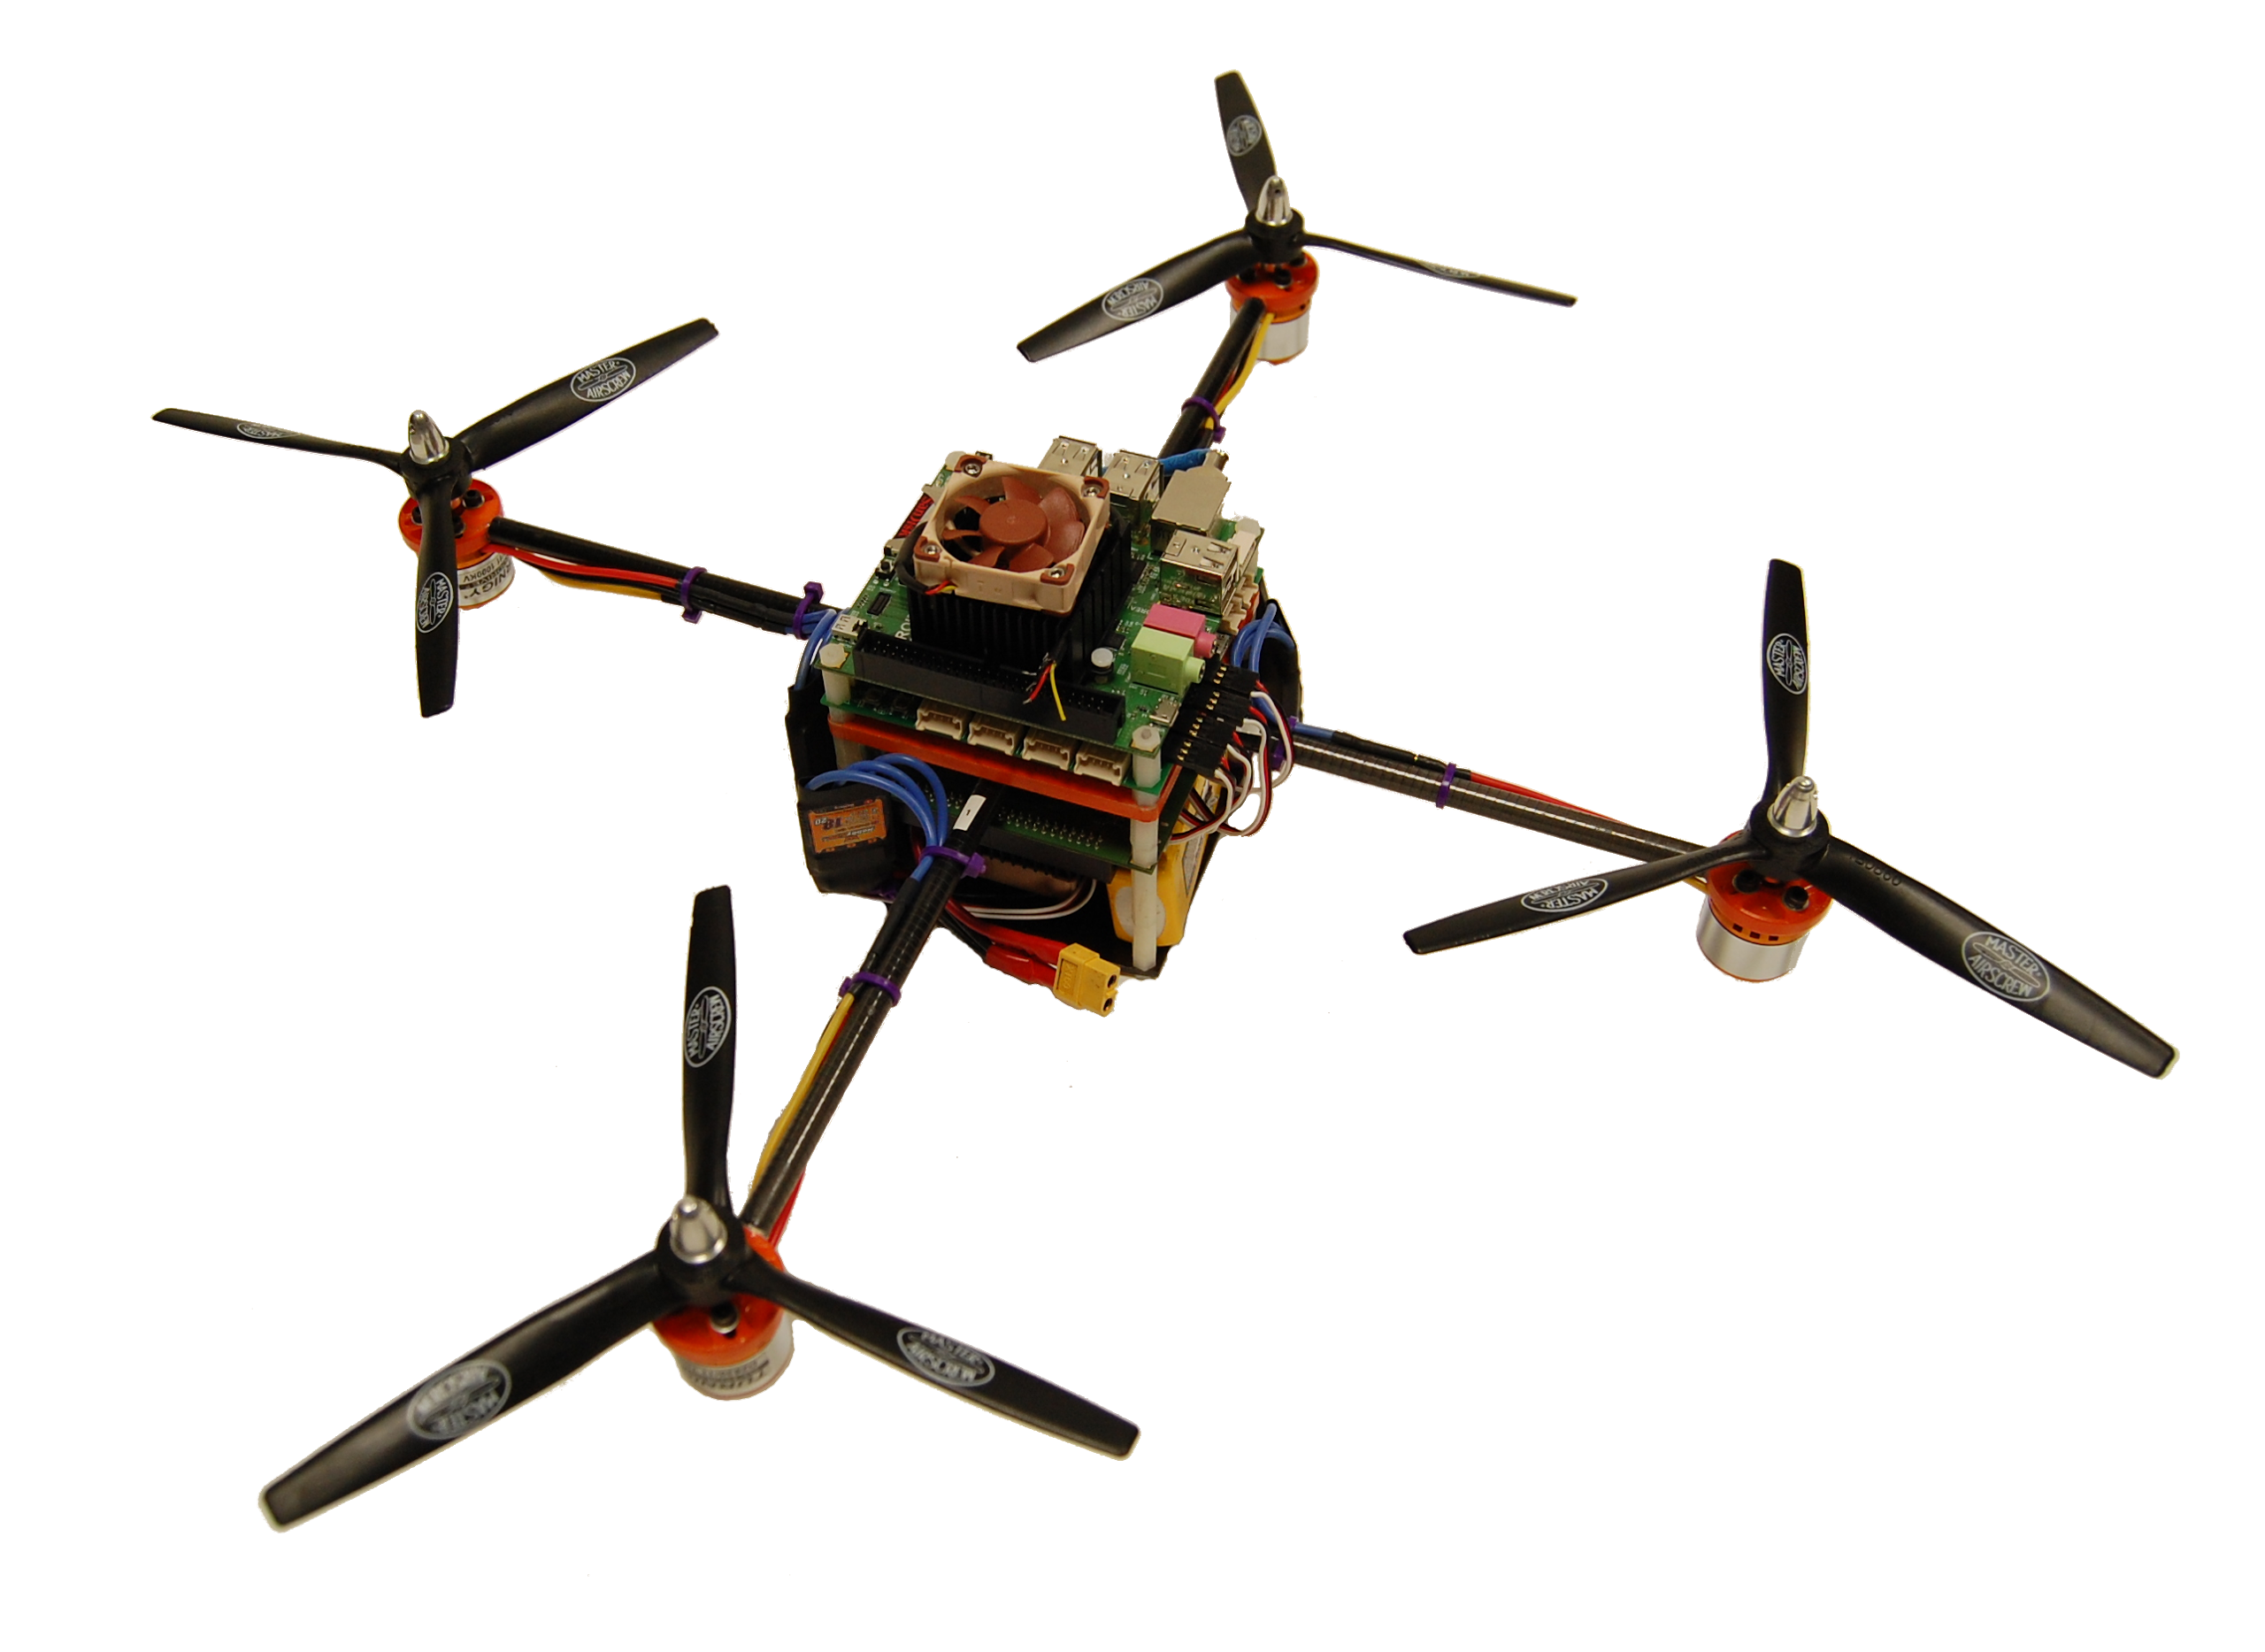
\includegraphics[width=5in]{quad}
  \caption{The 2014 quadrotor.}
\end{figure}

\section*{Technical Merit}
% IARC competition goal to further research in the area
% Full autonomy
% SLAM, optical flow, 
The stated goal of the IARC has always been to push the state-of-the-art of
aerial robotics forward. In past missions, this has involved indoor mapping and
exploration, long distance flying, and flight without onboard inertial
navigation systems. This year, the competition involves tracking a number of
ground robots, landing on top of them to cause them to change direction, and
herding them toward a single side of a rectangular arena. This will require
cooperation between software, electrical, and mechanical engineering students.

\subsection*{Software}
% Localization with optical flow
% TODO: how is this different from SLAM last year?
% TODO: mention PX4FLOW
There are two critical software challenges this year: localizing the aerial
vehicle in the arena and path planning. Last year, we used SLAM to both localize
and map our environment. This year, no mapping is necessary. We merely need to
localize the robot in the arena. We plan to use a technique called optical flow
to track our movement relative to the ground. We will use the Pixhawk PX4FLOW
sensor module, which contains all the hardware and software needed for optical
flow.

% Ground robot targeting

% Path planning and optimization
We are developing a simulator to test path planning algorithms. This simulator
will allow us to rapidly prototype planning algorithms and test them without the
need for physical hardware. This greatly lowers the barrier to entry for
development and increases the pace of the development cycle.
% TODO: reword independent of sensor noise

% Flight control
% TODO: use colon:
In addition to these challenges, we will be making revisions to our flight
control code: we will develop a method for tuning our configuration parameters
quantitatively, and will finalize the interface between the flight controller
and the onboard ODROID processing units.

\subsection*{Electrical}
% Flight control board revisions
We plan to make major revisions to our flight control board from last year to
allow for additional sensors and multiple rotor configurations. Last year, we
noticed that any flex applied to our flight control board would greatly increase
the error in our gyroscope and accelerometer readings. This year, we plan to
increase the thickness of our board to combat this issue, in addition to
optimizing the board for size and weight.
% TODO: Technically describe, microelectromechanical

% Kill switch mechanism
We will also be designing a kill switch per IARC rules. This kill switch will be
activated remotely over an XBee, and will immediately cut power to the motors.
We are investigating solid state relays for this purpose.

% XBee/flight control integration
% TODO: explain in first few sentences, not last few
We are also working on a wireless communication system that will allow us to
control the vehicle manually with a joystick connected to a host computer for
testing purposes. This can make use of the same XBee wireless module as the
kill switch. It must transmit commands from a joystick on the host computer to
the aerial vehicle, which must then act accordingly.

\subsection*{Mechanical}
% Carbon fiber propeller guard
% Landing gear
% TODO: what does safety and durability mean?
One of the biggest issues with our chassis last year was safety. The spinning
propellers had no protective shielding to prevent injury to misplaced fingers,
or to prevent damage from bumping into obstacles. We are adding a carbon fiber
propeller guard for safety and durability. We will also be constructing a carbon
fiber landing gear that will be responsible for triggering ground robots and
reducing chassis load on landings.
% TODO: not aid, do

% Sensor mountings
We will be investigating multiple optical flow sensor mounting strategies. The
mount will need to keep the sensor safe as well as provide it with a wide
unobstructed view of the arena.

% Ground robot triggering
Ground robots are to be triggered by magnets on the bottom of the aerial
vehicle. We will need to determine how best to design the triggering mechanism.
It will have to be lightweight, and allow us to land on ground robots without
upsetting the balance of the aerial vehicle. Ground robots may also be triggered
by landing in front of them, so we will need to ensure the chassis can survive
being repeatedly bumped by ground robots.

\section*{Broader Impact}
% Demonstrations Outreach
The OSU Autonomous Aerial Robotics Team is a learning experience for all those
involved. There are few other opportunities for students to participate in such
such a large interdisciplinary project, and to be on the forefront of research
in their field.

The team has functioned as a great springboard for those looking to start their
careers in robotics. Several team members have gone on to work for industry
leaders like SpaceX and Concept Systems, as well as the Dynamic Robotics
Laboratory and the Robotic Decision Making Laboratory at OSU.

% TODO: provide examples
% TODO: impact on STEM at OSU, what it's gonna do to the world
The team has also been involved in a number of outreach programs to get more
students involved in robotics. We presented at the Beaver Community Fair and the
OSU Engineering Expo, and gave a tour to students from Crescent Valley High
School. We have also demonstrated our aerial robots at numerous other events.

\section*{Budget}

\subsection*{Proposed from Robotics Club}

\begin{tabularx}{\textwidth}{ Xlrrr }
  \toprule
  Details                           & Quantity & Item cost (\$) & Total cost (\$) \\
  \midrule
  % TODO: add up real fc board costs
  Flight control rev. 3             & 4        & 100.00         &   400.00 \\
  Flight control rev. 4             & 4        & 120.00         &   480.00 \\
  Kill switch components            & 10       & 30.00          &   300.00 \\
  Propellers                        &          &                &   100.00 \\
  Landing gear materials            & 3        & 100.00         &   300.00 \\
  Misc. hardware                    &          &                &   500.00 \\
  Misc. electronics                 &          &                &   500.00 \\

  \textsc{Total Projected Cost}     &          &                & \fbox{2,580.00} \\
  \bottomrule                
\end{tabularx}

\subsection*{Proposed from Oregon NASA Space Grant}

\begin{tabularx}{\textwidth}{ Xlrrr }
  \toprule
  Details                           & Quantity & Item cost (\$) & Total cost (\$) \\
  \midrule
  % TODO: add up real fc board costs
  Camera mount                      & 3        & 50.00          & 150.00 \\
  Triggering Mechanism              & 3        & 50.00          & 150.00 \\
  Travel                            &          &                & 2,500.00 \\

  \textsc{Total Projected Cost}     &          &                & \fbox{2,800.00} \\
  \bottomrule                
\end{tabularx}

\begin{landscape}
\section*{Schedule}

\begin{gantt}[xunitlength=1.3cm,fontsize=\small,drawledgerline=true]{19}{12}
  \begin{ganttitle}
    \titleelement{2013}{3}
    \titleelement{2014}{9}
  \end{ganttitle}
  \begin{ganttitle}
    \titleelement{Sep}{1}
    \titleelement{Oct}{1}
    \titleelement{Nov}{1}
    \titleelement{Dec}{1}
    \titleelement{Jan}{1}
    \titleelement{Feb}{1}
    \titleelement{Mar}{1}
    \titleelement{Apr}{1}
    \titleelement{May}{1}
    \titleelement{Jun}{1}
    \titleelement{Jul}{1}
    \titleelement{Aug}{1}
  \end{ganttitle}

  % Software
  \ganttbar[color=blue]{Select sensors}{0}{1}
  \ganttbarcon[color=blue]{Off-board sensor functionality}{1}{1}
  \ganttbarcon[color=blue]{Autonomous position hold}{3}{3}
  \ganttbar[color=blue]{Ground robot tracking}{4}{3}
  \ganttbar[color=blue]{IARC simulator}{0}{3}
  \ganttbarcon[color=blue]{Path planning}{3}{5}
  \ganttbarcon[color=blue]{Onboard path planning integration}{8}{2}

  % Electrical
  \ganttbar[color=green]{Flight control revision}{0}{4}
  \ganttbar[color=green]{Kill switch}{3}{4}
  \ganttbar[color=green]{Remote control}{6}{4}

  % Mechanical
  \ganttbar[color=orange]{Propeller shroud}{0}{3}
  \ganttbar[color=orange]{Camera mount}{2}{3}
  \ganttbar[color=orange]{Landing gear}{4}{3}
  \ganttbar[color=orange]{Magnetic triggering mechanism}{6}{3}

  \ganttmilestone[color=cyan]{Autonomous flight}{10}
  \ganttbar{Integration testing}{10}{1}
  \ganttmilestone[color=red]{Competition}{11}
\end{gantt}
\end{landscape}

\section*{Appendix}

\begin{description}
  \item[IARC] International Aerial Robotics Competition
  \item[Optical Flow] A technique in which sequential video frames are compared
    to track moving features.
  \item[ODROID] A single-board computer used for vision and navigation
    processing on board the aerial vehicle.
  \item[XBee] A family of easy-to-use wireless radio modules.
  \item[SLAM] Simultaneous localization and mapping. A technique used by robots
    to build up a map of an unknown environment while keeping track of its
    position.
\end{description}

\end{document}
